%% ============================================================
%% TP S3 DUT -- Développement d'une nouvelle méthodologie ML
%% ============================================================
\documentclass[a4paper,fleqn]{cas-sc}

\usepackage[T1]{fontenc}
\usepackage[french]{babel}
\usepackage[authoryear,longnamesfirst]{natbib}
\usepackage{graphicx}
\usepackage{hyperref}
\usepackage{amsmath,amsfonts,amssymb}
\usepackage{booktabs}
\usepackage{xcolor}
\usepackage{tikz}
\usetikzlibrary{arrows.meta,positioning,shapes.geometric}
\usepackage{algorithm}
\usepackage{algpseudocode}
\graphicspath{{figures/}}

\algrenewcommand\algorithmicrequire{\textbf{Entrées :}}
\algrenewcommand\algorithmicensure{\textbf{Sortie :}}
\algrenewcommand\algorithmicfor{\textbf{pour}}
\algrenewcommand\algorithmicdo{\textbf{faire}}
\algrenewcommand\algorithmicif{\textbf{si}}
\algrenewcommand\algorithmicthen{\textbf{alors}}
\algrenewcommand\algorithmicelse{\textbf{sinon}}
\algrenewcommand\algorithmicreturn{\textbf{retourner}}
\renewcommand{\algorithmicname}{Algorithme}

\newtheorem{theorem}{Proposition}

\begin{document}
\let\WriteBookmarks\relax
\def\floatpagepagefraction{1}
\def\textpagefraction{.001}

%% ===== TITRE COURT & AUTEUR =====
\shorttitle{Cascade à confiance contrôlée}
\shortauthors{Oualache}

\title [mode = title]{Développement d'une nouvelle méthodologie de Machine Learning~:
\textit{Cascade à confiance contrôlée avec révision humaine pour la détection de messages nuisibles en français}}
\tnotemark[1]
\tnotetext[1]{Travaux Pratiques -- Module Intelligence Artificielle, DUT IDRS S3, Pr. Chaimae Boulahia. Année universitaire 2026--2027.}

\author[1]{Said Oualache}
\ead{said.oualache@uit.ac.ma}
\ead[url]{https://github.com/SaidOualache/detection-messages-nuisibles-fr}

\credit{Conception méthodologique, Implémentation Python, Analyse expérimentale}

\affiliation[1]{organization={Département Mathématiques et Informatique -- DUT-IDRS-S3},
    addressline={École Supérieure de Technologie},
    city={Kénitra},
    postcode={14000},
    state={Université Ibn Tofaïl},
    country={Maroc}}

%% ===== RÉSUMÉ =====
\begin{abstract}
Les plateformes en ligne filtrent automatiquement les messages nuisibles, mais un classifieur unique
se trompe sur les cas ambigus, et une erreur n'a pas le même coût selon sa nature. Nous proposons une
\textbf{cascade à confiance contrôlée} pour le français : une régression logistique sur
TF-IDF répond seule lorsque sa confiance dépasse un seuil $\tau_1$ ; sinon un classifieur des $k$ plus
proches voisins donne son avis s'il est assez sûr (seuil $\tau_2$) ; les cas restants sont confiés à un
modérateur humain. Les deux seuils sont choisis sur un jeu de validation en minimisant un coût moyen qui
distingue le faux blocage, le message nuisible raté et l'envoi à un humain. Sur le \textit{French Hate
Speech Superset} (17\,897 messages après nettoyage, 24\,\% nuisibles), avec 5 exécutions
indépendantes, la cascade obtient un coût de $0.356 \pm 0.014$ contre $0.462 \pm 0.031$ pour la régression
logistique seule et $0.923 \pm 0.025$ pour les $k$ plus proches voisins seuls, en envoyant $40\,\%$ des
messages à un humain. Une ablation montre toutefois que ce gain provient de la zone de révision
humaine et non du second classifieur : « régression logistique + humain » atteint le même coût
($0.355 \pm 0.014$).
\end{abstract}

%% ===== MOTS-CLÉS =====
\begin{keywords}
détection de contenus nuisibles \sep classification de texte \sep cascade de classifieurs
\sep option de rejet \sep apprentissage sensible aux coûts \sep français
\end{keywords}

%% ===== POINTS CLÉS DU TP (Highlights) =====
\begin{highlights}
\item Architecture originale : cascade régression logistique, $k$-NN, humain, avec seuils de confiance choisis par un coût explicite.
\item Mise en œuvre complète en Python (scikit-learn), reproductible, code public sur GitHub.
\item Comparaison quantitative avec deux méthodes de référence et une ablation, sur 5 exécutions indépendantes.
\end{highlights}

\maketitle

%% ===== CORPS DU DOCUMENT =====
\section{Introduction}

Les réseaux sociaux et les assistants conversationnels doivent repérer automatiquement les messages
nuisibles (haine, insultes, menaces, racisme, sexisme). Un classifieur unique rencontre deux limites.
D'abord, il est parfois peu sûr de lui : forcer une réponse sur ces cas produit des erreurs.
Ensuite, les deux erreurs possibles ne se valent pas : bloquer à tort un message inoffensif gêne un
utilisateur, mais laisser passer un message nuisible peut blesser quelqu'un.

Nous proposons une \textbf{cascade à confiance contrôlée}. Un modèle rapide (régression logistique)
décide seul lorsqu'il est sûr de lui. Sinon, un second modèle ($k$ plus proches voisins) donne son
avis, et si le doute persiste, le message est transmis à un modérateur humain. Les seuils de confiance
ne sont pas fixés à la main : ils sont choisis pour minimiser un coût moyen qui tient compte de la
gravité de chaque type d'erreur et du coût de la révision humaine.

Les contributions de ce travail sont :
\begin{enumerate}
    \item Une formalisation mathématique claire de la cascade et du choix des seuils par un coût (Sec.~\ref{sec:metho}) ;
    \item Une implémentation reproductible et documentée sur des données françaises (Sec.~\ref{sec:impl}) ;
    \item Une évaluation rigoureuse sur 5 exécutions, avec deux références et une ablation, qui montre
    où se situe réellement le gain (Sec.~\ref{sec:res} et~\ref{sec:disc}).
\end{enumerate}

\section{Positionnement et travaux existants}

\paragraph{Option de rejet et coûts.}
\citet{Chow1970} montre que la règle optimale d'une classification avec option de rejet consiste à
refuser de décider lorsque la probabilité a posteriori maximale est trop faible, et qu'un seuil unique
règle le compromis entre erreurs et rejets. \citet{Elkan2001} montre que, lorsque les erreurs ont des
coûts différents, la décision optimale dépend du rapport de ces coûts. Notre zone de révision humaine est
une option de rejet, et notre coût moyen (Sec.~\ref{sec:cout}) combine ces deux idées.

\paragraph{Détection de contenus nuisibles en français.}
Les ressources françaises sont moins nombreuses qu'en anglais. \citet{Delaval2025} publient
ToxiFrench, 53\,622 commentaires français avec un jeu d'évaluation équilibré, annotés par un procédé
semi-automatique qui limite l'annotation manuelle à 10\,\%. \citet{Tonneau2024} fusionnent les jeux de
données de haine disponibles en un « superset » par langue, dont la version française est utilisée ici.
Les modèles de langue comme CamemBERT \citep{Martin2020} constituent le candidat naturel pour un
second étage plus puissant (voir les perspectives).

\paragraph{Approches hybrides et en cascade.}
\citet{Kumar2025} combinent une régression logistique et un BERT affiné sur le jeu anglais Jigsaw, avec
des seuils par catégorie choisis par recherche sur grille pour maximiser le F1.
\citet{ElBahnasawi2025} proposent un cadre en trois couches : un préfiltre à règles (lexiques et
expressions régulières), puis un BERTweet adapté par LoRA. Ces travaux portent sur l'anglais.

\paragraph{Notre différence.} Nous travaillons sur le français ; nos seuils sont choisis par un coût qui
inclut explicitement la révision humaine ; la cascade a deux seuils et une zone humaine dont nous
mesurons la part ; le second étage est léger (CPU) ; et nous incluons une ablation qui isole l'apport de
chaque étage. Nous ne prétendons pas que l'idée de cascade soit nouvelle.

\section{Méthodologie proposée}
\label{sec:metho}

\subsection{Notations et formulation mathématique}

Soit $\mathcal{D} = \{(x_i, y_i)\}_{i=1}^{N}$ un jeu de messages $x_i$ avec leur étiquette
$y_i \in \{0,1\}$ ($1$ : nuisible, $0$ : sûr). Un message est transformé en vecteur
$\varphi(x) \in \mathbb{R}^{d}$ par TF-IDF \citep{Salton1988}. Nous concaténons deux vectorisations,
chacune normalisée en norme $\ell_2$ : l'une sur les mots et bigrammes, l'autre sur les $n$-grammes de
caractères (de 2 à 5). Pour un terme $t$ de fréquence $\mathrm{tf}(t,x)$ dans le message $x$ et de
fréquence documentaire $\mathrm{df}(t)$ :
\begin{equation}
\mathrm{tfidf}(t,x) = \bigl(1 + \ln \mathrm{tf}(t,x)\bigr)\,\Bigl(\ln\frac{1+N}{1+\mathrm{df}(t)} + 1\Bigr).
\end{equation}

\paragraph{Étage 1 : régression logistique.} Elle donne la probabilité d'être nuisible
\begin{equation}
p_1(x) = \sigma\bigl(w^{\top}\varphi(x) + b\bigr), \qquad \sigma(z) = \frac{1}{1+e^{-z}},
\label{eq:rl}
\end{equation}
où $(w,b)$ minimisent une perte logistique pondérée avec pénalité $\ell_2$ :
\begin{equation}
\min_{w,b}\; \tfrac{1}{2}\lVert w\rVert^{2} + C\sum_{i=1}^{N} \omega_{y_i}\,\Bigl[-y_i\ln p_1(x_i) - (1-y_i)\ln\bigl(1-p_1(x_i)\bigr)\Bigr],
\label{eq:loss}
\end{equation}
avec $C=1$ et des poids équilibrés $\omega_c = N/(2N_c)$ ($N_c$ : nombre d'exemples de la classe $c$), qui
compensent la rareté des messages nuisibles.

\paragraph{Étage 2 : $k$ plus proches voisins.} Avec la similarité cosinus et $\mathcal{N}_K(x)$ l'ensemble
des $K$ messages d'entraînement les plus proches de $x$ \citep{CoverHart1967},
\begin{equation}
p_2(x) = \frac{1}{K}\sum_{i\in\mathcal{N}_K(x)} y_i .
\label{eq:knn}
\end{equation}

\paragraph{Confiance et règle de la cascade.} La confiance d'un étage est la probabilité de la classe
qu'il choisit :
\begin{equation}
c_j(x) = \max\bigl(p_j(x),\,1-p_j(x)\bigr) \in [0.5,\,1], \qquad j\in\{1,2\}.
\end{equation}
Avec deux seuils $\tau_1,\tau_2\in[0.5,1]$, la décision de la cascade est
\begin{equation}
\hat{y}(x) =
\begin{cases}
\mathbb{1}\,[\,p_1(x)\ge 0.5\,] & \text{si } c_1(x)\ge\tau_1,\\[2pt]
\mathbb{1}\,[\,p_2(x)\ge 0.5\,] & \text{si } c_1(x)<\tau_1 \text{ et } c_2(x)\ge\tau_2,\\[2pt]
\bot\ (\text{révision humaine}) & \text{sinon.}
\end{cases}
\label{eq:cascade}
\end{equation}
La figure~\ref{fig:pipeline} résume le fonctionnement.

\begin{figure}[t]
\centering
\begin{tikzpicture}[node distance=6mm, >=Stealth,
  boite/.style={draw, rounded corners, align=center, minimum height=7mm, inner sep=3pt, fill=gray!8},
  test/.style={draw, diamond, aspect=3, align=center, inner sep=0pt, fill=orange!12},
  fin/.style={draw, rounded corners, align=center, minimum height=7mm, fill=teal!15},
  humain/.style={draw, rounded corners, align=center, minimum height=7mm, fill=red!12}]
\node[boite] (x) {Message $x$ (français)};
\node[boite, below=of x] (tfidf) {Étape 0 : TF-IDF mots + caractères, $\varphi(x)$};
\node[boite, below=of tfidf] (rl) {Étape 1 : régression logistique, $p_1(x)$ et $c_1(x)$};
\node[test, below=of rl] (t1) {$c_1(x)\ge\tau_1$ ?};
\node[fin, right=14mm of t1] (d1) {Décision RL};
\node[boite, below=of t1] (knn) {Étape 2 : $k$-NN (cosinus), $p_2(x)$ et $c_2(x)$};
\node[test, below=of knn] (t2) {$c_2(x)\ge\tau_2$ ?};
\node[fin, right=14mm of t2] (d2) {Décision $k$-NN};
\node[humain, below=of t2] (h) {Étape 3 : modérateur humain};
\draw[->] (x) -- (tfidf);
\draw[->] (tfidf) -- (rl);
\draw[->] (rl) -- (t1);
\draw[->] (t1) -- node[above] {oui} (d1);
\draw[->] (t1) -- node[left] {non} (knn);
\draw[->] (knn) -- (t2);
\draw[->] (t2) -- node[above] {oui} (d2);
\draw[->] (t2) -- node[left] {non} (h);
\end{tikzpicture}
\caption{Fonctionnement de la cascade à confiance contrôlée.}
\label{fig:pipeline}
\end{figure}

\subsection{Coût moyen et choix des seuils}
\label{sec:cout}

Parmi les messages décidés par les modèles, soient $\mathrm{FP}$ le nombre de messages sains bloqués à
tort et $\mathrm{FN}$ le nombre de messages nuisibles laissés passer ; soit $H$ le nombre de messages
envoyés à un humain (que nous supposons toujours bien classés). Le coût moyen sur $n$ messages est
\begin{equation}
J(\tau_1,\tau_2) = \frac{a\cdot\mathrm{FP} + b\cdot\mathrm{FN} + h\cdot H}{n},
\label{eq:cout}
\end{equation}
avec $a=1$ (faux blocage), $b=5$ (message nuisible raté) et $h=0.5$ (révision humaine). Ces valeurs sont
des hypothèses qui traduisent un ordre : rater un message nuisible est plus grave que bloquer à tort,
et faire relire coûte moins cher qu'une erreur sans être gratuit. Leur influence est étudiée en
section~\ref{sec:disc}. Les seuils sont choisis sur le jeu de validation, parmi la grille
$\mathcal{T}=\{0.50, 0.55, \dots, 1.00\}$ :
\begin{equation}
(\tau_1^{*},\tau_2^{*}) = \operatorname*{arg\,min}_{(\tau_1,\tau_2)\in\mathcal{T}^2} J_{\mathrm{val}}(\tau_1,\tau_2),
\label{eq:argmin}
\end{equation}
en retenant le premier minimum rencontré en cas d'égalité. Le jeu de test n'intervient jamais dans ce choix.

\subsection{Algorithmes}

\begin{algorithm}[t]
\caption{Apprentissage et choix des seuils}
\label{alg:train}
\begin{algorithmic}[1]
\Require $\mathcal{D}_{\mathrm{train}}$, $\mathcal{D}_{\mathrm{val}}$, coûts $(a,b,h)$, grille $\mathcal{T}$, entier $K$
\State Ajuster le TF-IDF sur $\mathcal{D}_{\mathrm{train}}$ et calculer $\varphi(x)$ pour tout message
\State Entraîner la régression logistique pondérée (éq.~\ref{eq:loss}) sur $\mathcal{D}_{\mathrm{train}}$
\State Mémoriser $\mathcal{D}_{\mathrm{train}}$ pour le $k$-NN
\State Calculer $p_1(x)$ et $p_2(x)$ pour chaque $x\in\mathcal{D}_{\mathrm{val}}$
\For{$(\tau_1,\tau_2)\in\mathcal{T}^2$}
    \State Appliquer la règle (éq.~\ref{eq:cascade}) à $\mathcal{D}_{\mathrm{val}}$ et calculer $J_{\mathrm{val}}(\tau_1,\tau_2)$
\EndFor
\State $(\tau_1^{*},\tau_2^{*}) \gets \arg\min J_{\mathrm{val}}$
\Ensure TF-IDF, régression logistique, $\mathcal{D}_{\mathrm{train}}$, $(\tau_1^{*},\tau_2^{*})$
\end{algorithmic}
\end{algorithm}

\begin{algorithm}[t]
\caption{Décision pour un nouveau message $x$}
\label{alg:predict}
\begin{algorithmic}[1]
\State $p_1 \gets p_1(x)$
\If{$\max(p_1,1-p_1)\ge\tau_1^{*}$} \Return $\mathbb{1}[p_1\ge 0.5]$
\EndIf
\State $p_2 \gets p_2(x)$ \Comment{le $k$-NN n'est appelé que pour les cas douteux}
\If{$\max(p_2,1-p_2)\ge\tau_2^{*}$} \Return $\mathbb{1}[p_2\ge 0.5]$
\EndIf
\State \Return envoyer à un modérateur humain
\end{algorithmic}
\end{algorithm}

\subsection{Propriétés}

\begin{theorem}[Cas limites de la cascade]
\label{thm:lim}
(i) Pour $\tau_1=0.5$, la cascade coïncide avec la régression logistique seule, quel que soit $\tau_2$.
(ii) Pour $\tau_2>1$, elle coïncide avec le système « régression logistique + humain ».
(iii) Par conséquent, le coût de validation minimal de la cascade est inférieur ou égal à celui de la
régression logistique seule ; et, si la grille contient une valeur $\tau_2>1$, inférieur ou égal à celui de
« régression logistique + humain ».
\end{theorem}
\begin{proof}
Comme $c_1(x)\ge 0.5$ pour tout $x$, la condition $c_1(x)\ge 0.5$ est toujours vraie : le premier cas
de l'équation~\eqref{eq:cascade} s'applique toujours, d'où (i). Comme $c_2(x)\le 1$, la condition
$c_2(x)\ge\tau_2$ est fausse si $\tau_2>1$ : le deuxième cas n'est jamais atteint, d'où (ii). Enfin, ces
deux systèmes correspondent à des couples de la grille (resp. de la grille élargie), et le minimum d'un
ensemble est inférieur ou égal à chacun de ses éléments, d'où (iii).
\end{proof}
Cette garantie ne concerne que la validation : sur le jeu de test, rien n'assure que la cascade
reste meilleure. Dans nos expériences, nous évaluons « régression logistique + humain » séparément, avec
un seuil $\tau_2=1.01$.

\section{Implémentation et protocole expérimental}
\label{sec:impl}

\subsection{Jeu de données et pré-traitement}

Nous utilisons le \textit{French Hate Speech Superset} \citep{Tonneau2024}, qui rassemble des messages
issus de cinq corpus publics (CONAN, MLMA, un corpus de sexisme sur des tweets français,
CyberAgressionAdo et un corpus de propos racistes sur des tweets français). Les étiquettes d'origine,
hétérogènes, y sont binarisées (haineux ou non) et les noms d'utilisateur et liens sont remplacés par des
marqueurs. L'accès au jeu de données est restreint et soumis à demande ; il n'est donc pas redistribué
dans notre dépôt.

Le fichier contient 18\,071 messages. Nous gardons le texte et l'étiquette, puis nous supprimons les
valeurs manquantes, les doublons exacts et les textes présents avec des étiquettes contradictoires, ce
qui laisse $N=17\,897$ messages, dont 24\,\% sont nuisibles. La vectorisation TF-IDF (Sec.~\ref{sec:metho}) joue
le rôle de normalisation des données. Le découpage est stratifié : $70\,\%$ pour l'entraînement
(12\,527 messages), $15\,\%$ pour la validation (2\,685) et $15\,\%$ pour le test (2\,685). Le vocabulaire
TF-IDF est appris sur l'entraînement seul.

\subsection{Environnement technique}

\begin{itemize}
    \item Langage : Python 3.14.3
    \item Bibliothèques : scikit-learn \citep{Pedregosa2011}, pandas, SciPy 1.18.0, Matplotlib % TODO : ajouter les versions de scikit-learn, pandas et Matplotlib
    \item Matériel : ordinateur portable Dell Latitude 5420, Windows 11 Pro, processeur Intel Core de 11\textsuperscript{e} génération, 16~Go de RAM, sans GPU % TODO : remplacer par le nom exact du processeur
    \item Reproductibilité : 5 exécutions avec les graines 42, 43, 44, 45 et 46 (découpage des données) ; code et instructions sur le dépôt GitHub.
\end{itemize}

\subsection{Hyper-paramètres}

TF-IDF : mots et bigrammes (fréquence documentaire minimale 2, fréquence sous-linéaire) et $n$-grammes de
caractères de 2 à 5 (\texttt{char\_wb}). Régression logistique : $C=1$, poids équilibrés, 1000 itérations
au plus. $k$-NN : $K=15$ voisins, distance cosinus, calcul exhaustif. Grille de seuils $\mathcal{T}$ de $0.50$ à
$1.00$ par pas de $0.05$. Coûts $(a,b,h)=(1,5,0.5)$.

\paragraph{Justification des choix.}
La régression logistique est la version « classification » de la régression
linéaire vue en cours : elle est rapide et sa sortie $p_1(x)$ est directement
une probabilité, donc une confiance. Le $k$-NN, aussi vu en cours, raisonne
différemment (par exemples proches et non par poids linéaires), ce qui le rend
a priori complémentaire. Le TF-IDF sur les mots capte le vocabulaire, et celui
sur les caractères reste robuste aux fautes, allongements et insultes
déformées. $K=15$ (impair, pour éviter les égalités), $C=1$ et le pas de $0.05$
ont été fixés a priori et non optimisés ; étudier leur influence est une
perspective. Les poids de classes équilibrés compensent la rareté des messages
nuisibles ($24\,\%$), et les coûts $(a,b,h)$ traduisent un ordre de gravité
(section~\ref{sec:cout}) dont la sensibilité est étudiée en section~\ref{sec:disc}.

\subsection{Systèmes comparés}

Nous comparons quatre systèmes sur les mêmes découpages : la régression logistique seule (\textsc{Référence A}),
les $k$-NN seuls (\textsc{Référence B}), « régression logistique + humain » (la cascade sans le $k$-NN,
ablation) et notre cascade complète (\textsc{Proposée}). Pour « régression logistique + humain », le seuil
$\tau_1$ est choisi par le même procédé et $\tau_2=1.01$.

\subsection{Métriques d'évaluation}

\begin{equation}
\text{Accuracy} = \frac{\text{TP}+\text{TN}}{\text{TP}+\text{TN}+\text{FP}+\text{FN}}, \quad
\text{Précision} = \frac{\text{TP}}{\text{TP}+\text{FP}}, \quad
\text{Rappel} = \frac{\text{TP}}{\text{TP}+\text{FN}}, \quad
F_1 = 2 \cdot \frac{\text{Précision} \cdot \text{Rappel}}{\text{Précision} + \text{Rappel}}.
\end{equation}
La précision et le rappel concernent la classe « nuisible ». Le $F_1$ \textit{macro} est la moyenne des
$F_1$ des deux classes, ce qui évite que la classe majoritaire masque les performances sur la classe
rare. Nous ajoutons le taux de faux positifs $\mathrm{FP}/(\mathrm{FP}+\mathrm{TN})$, la part de messages
envoyés à un humain $H/n$, le coût $J$ (éq.~\ref{eq:cout}) et le temps de prédiction par message (modèles
seuls, sans la vectorisation, mesuré sur CPU). Pour les systèmes avec humain, l'accuracy, la précision, le
rappel, le $F_1$ et les faux positifs ne portent que sur les messages décidés par les modèles ; le coût
$J$ est donc la comparaison la plus juste.

\section{Résultats et analyse}
\label{sec:res}

Les tableaux~\ref{tbl:res1} et~\ref{tbl:res2} résument les performances sur le jeu de test.

\begin{table}[width=.95\linewidth,cols=5,pos=h]
\caption{Qualité des décisions (jeu de test). Moyenne $\pm$ écart-type sur 5 exécutions indépendantes.
RL : régression logistique. Précision et rappel : classe « nuisible ».}
\label{tbl:res1}
\begin{tabular*}{\tblwidth}{@{} LLLLL @{} }
\toprule
Méthode & Accuracy (\%) & Précision (\%) & Rappel (\%) & $F_1$ macro (\%) \\
\midrule
Référence A : RL brute & 80.0 $\pm$ 1.0 & 56.4 $\pm$ 1.5 & 72.7 $\pm$ 2.3 & 74.9 $\pm$ 1.2 \\
Référence B : KNN brute & 79.6 $\pm$ 0.6 & 71.7 $\pm$ 3.0 & 25.0 $\pm$ 2.1 & 62.5 $\pm$ 1.4 \\
Ablation : RL + humain & 90.3 $\pm$ 2.4 & 72.9 $\pm$ 4.7 & 82.7 $\pm$ 2.0 & 85.6 $\pm$ 2.5 \\
\textbf{Notre cascade} & \textbf{90.0} $\pm$ 2.7 & 72.7 $\pm$ 5.1 & 80.7 $\pm$ 1.7 & 85.0 $\pm$ 2.7 \\
\bottomrule
\end{tabular*}
\end{table}

\begin{table}[width=.95\linewidth,cols=5,pos=h]
\caption{Erreurs, charge humaine, coût et temps (jeu de test). Moyenne $\pm$ écart-type sur 5 exécutions.
Le coût est celui de l'équation~\eqref{eq:cout}, plus bas est meilleur.}
\label{tbl:res2}
\begin{tabular*}{\tblwidth}{@{} LLLLL @{} }
\toprule
Méthode & Faux positifs (\%) & Envoyé à l'humain (\%) & Coût $J$ & Temps (ms/msg) \\
\midrule
Référence A : RL brute & 17.7 $\pm$ 0.6 & 0.0 & 0.462 $\pm$ 0.031 & 0.0014 $\pm$ 0.0002 \\
Référence B : KNN brute & 3.1 $\pm$ 0.4 & 0.0 & 0.923 $\pm$ 0.025 & 0.9962 $\pm$ 0.3690 \\
Ablation : RL + humain & 7.8 $\pm$ 2.4 & 44.0 $\pm$ 9.3 & \textbf{0.355} $\pm$ 0.014 & 0.0014 $\pm$ 0.0002 \\
\textbf{Notre cascade} & 7.8 $\pm$ 2.8 & 40.0 $\pm$ 11.2 & \textbf{0.356} $\pm$ 0.014 & 0.5212 $\pm$ 0.3294 \\
\bottomrule
\end{tabular*}
\end{table}

\paragraph{Interprétation.} Le coût de la cascade ($0.356$) est inférieur d'environ 23\,\% à celui de la
régression logistique seule ($0.462$) et bien inférieur à celui des $k$-NN seuls ($0.923$). L'écart avec la
régression logistique ($0.106$) est très supérieur aux écarts-types ($0.014$ et $0.031$), ce qui indique
une différence réelle et non un effet du hasard. La cascade réduit aussi les faux positifs, de $17.7\,\%$
à $7.8\,\%$, et son rappel sur la classe nuisible est de $80.7\,\%$ pour une précision de $72.7\,\%$.
Ces gains ont un prix : 40\,\% des messages sont renvoyés à un humain, avec une forte variabilité
($\pm 11.2$ points) selon le découpage. Son exactitude de $90.0\,\%$ ne concerne que les messages décidés par
les modèles ; si l'on exige une réponse pour tous les messages, la meilleure exactitude observée est
celle de la régression logistique brute, soit $80.0\,\%$.

Les $k$-NN seuls ont une bonne précision ($71.7\,\%$) mais un rappel de $25.0\,\%$ : ils laissent passer
trois messages nuisibles sur quatre, d'où un coût très élevé puisque ce type d'erreur coûte $5$.

\paragraph{Ablation.} La ligne « RL + humain » a un coût de $0.355$, contre $0.356$ pour la cascade : la différence
($0.001$) est quatorze fois plus petite que l'écart-type. Le second étage n'apporte donc aucun gain
mesurable, alors qu'il multiplie le temps de calcul par environ $370$ par rapport à la régression logistique
seule ($0.52$ contre $0.0014$ ms par message, sur CPU).

\paragraph{Seuils retenus.} Le seuil $\tau_2$ retenu vaut $0.95$ dans les 5 exécutions, et $\tau_1$ vaut respectivement
$0.75$, $0.80$, $0.65$, $0.70$ et $0.75$. La figure~\ref{fig:seuils} montre le coût moyen de validation pour
chaque couple de la grille : le minimum se trouve en $(0.75;\,0.95)$ (coût $0.366$), dans une large zone
verte, et pas sur un bord de la grille. Avec $K=15$ voisins, la confiance du $k$-NN ne peut valoir que
$8/15,\dots,15/15$ : exiger $c_2\ge 0.95$ revient à exiger que les $15$ voisins soient d'accord, et les colonnes
$0.95$ et $1.00$ de la figure sont identiques.

\begin{figure}[t]
\centering
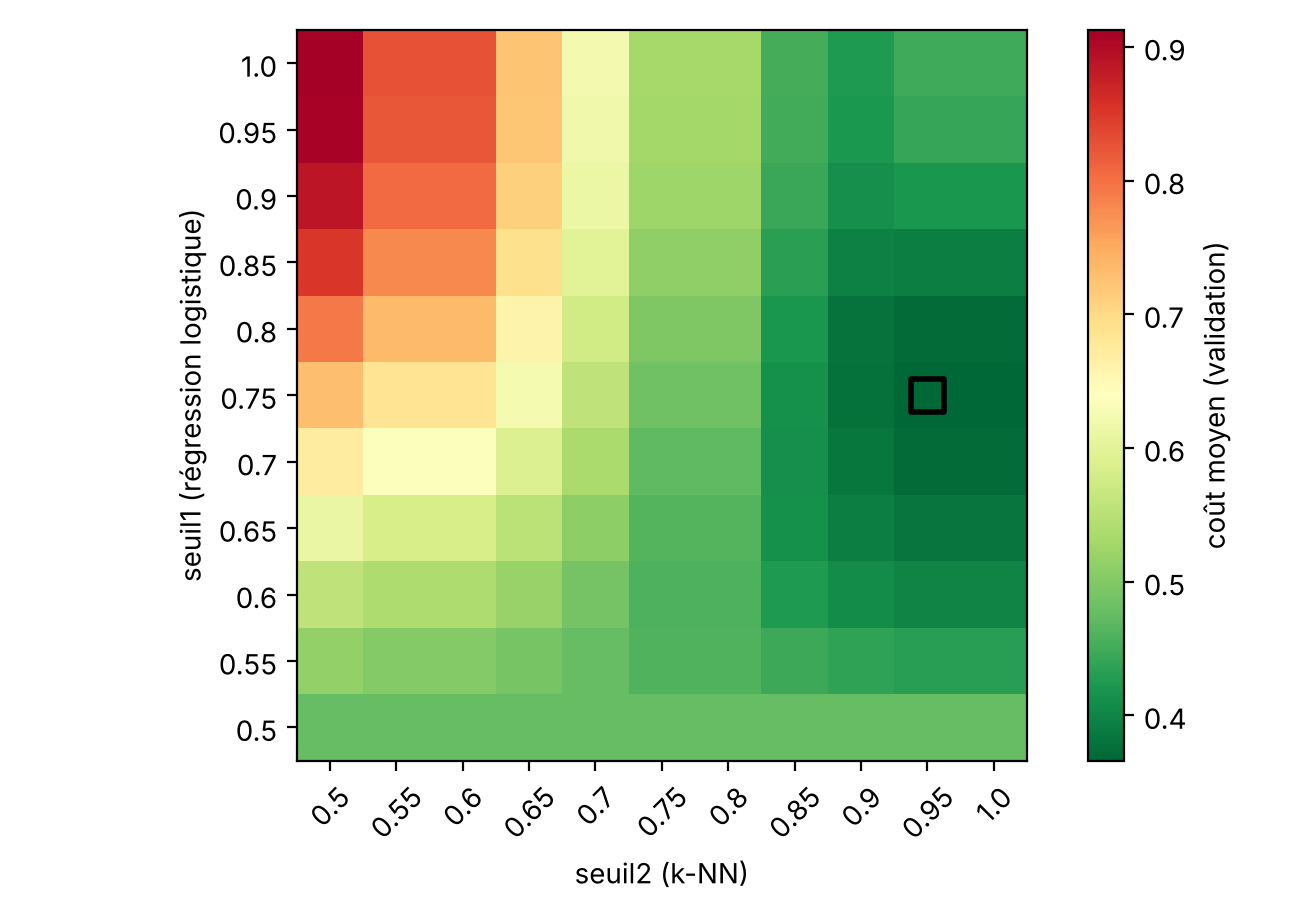
\includegraphics[width=.78\linewidth]{fig_seuils.png}
\caption{Coût moyen sur la validation (moyenne des 5 exécutions) pour chaque couple de seuils. Le carré
noir marque le minimum.}
\label{fig:seuils}
\end{figure}

\begin{figure}[t]
\centering
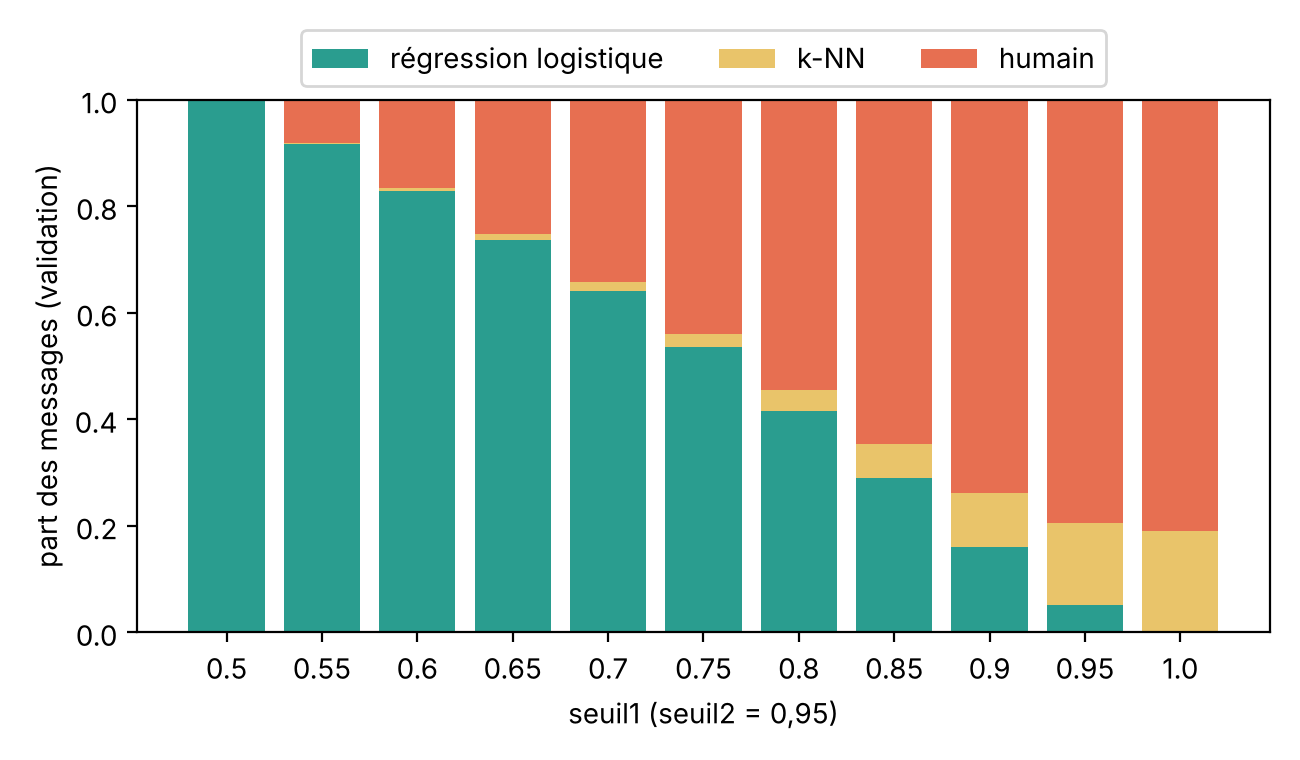
\includegraphics[width=.78\linewidth]{fig_decideurs.png}
\caption{Part des messages décidés par chaque étage selon $\tau_1$ (avec $\tau_2=0.95$, validation).
Pour $\tau_1=0.75$ : régression logistique 53.5\,\%, $k$-NN 2.6\,\%, humain 43.9\,\%.}
\label{fig:decideurs}
\end{figure}

\begin{figure}[t]
\centering
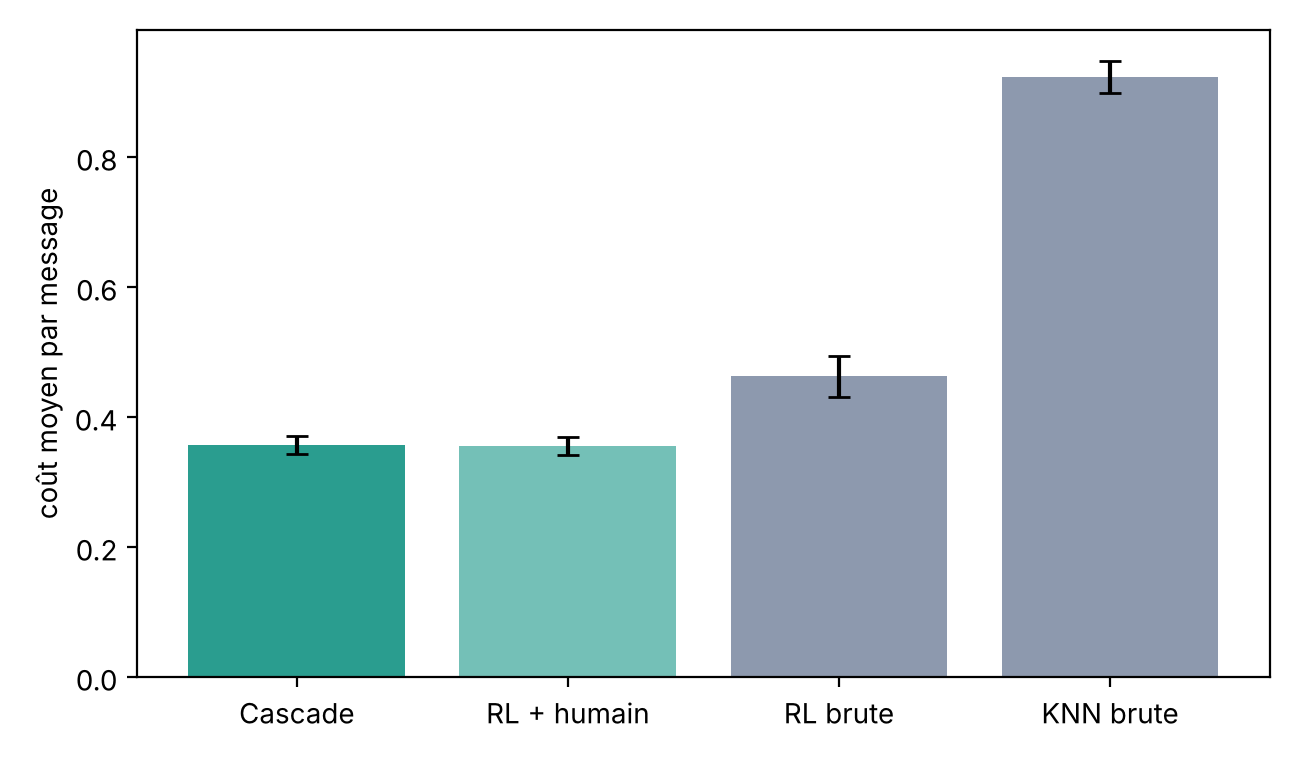
\includegraphics[width=.7\linewidth]{fig_cout.png}
\caption{Coût moyen par message sur le jeu de test (moyenne des 5 exécutions, barres : écart-type).}
\label{fig:cout}
\end{figure}

\section{Discussion}
\label{sec:disc}

Malgré ces résultats, plusieurs limitations doivent être soulignées.

\begin{enumerate}
    \item \textbf{Le $k$-NN n'apporte presque rien.} La figure~\ref{fig:decideurs} montre qu'à $\tau_1=0.75$ il ne
    décide que $2.6\,\%$ des messages : presque tout le reste va à l'humain. Une explication plausible, que nous
    n'avons pas vérifiée, est que dans un espace TF-IDF creux les voisins partagent peu de mots, et que,
    les messages nuisibles ne représentant que $24\,\%$ des données, la plupart des voisins sont sains :
    le $k$-NN prédit rarement « nuisible » (rappel de $25\,\%$) et son unanimité est rare. Un second étage ne peut
    aider que s'il sait quelque chose que le premier ignore.
    \item \textbf{Le gain dépend des coûts choisis.} Le tableau~\ref{tbl:sens} refait le choix des seuils avec d'autres
    coûts. Si la révision humaine coûte $h\ge 1$, la zone humaine disparaît ($5.8\,\%$ des messages pour $h=1$, $0\,\%$
    pour $h=2$) et la cascade rejoint la régression logistique seule. Si rater un message nuisible coûte peu ($b=2$), le gain est
    faible ($0.254$ contre $0.266$). Quand l'humain est très bon marché ($h=0.1$) ou que le message raté est très
    grave ($b=10$), « RL + humain » est même meilleure que la cascade ($0.100$ contre $0.120$, et $0.428$ contre $0.438$) :
    les décisions « sûres » du $k$-NN contiennent des erreurs qu'un humain aurait corrigées. Les valeurs $(1,5,0.5)$ sont des
    hypothèses, pas des mesures.
    \item \textbf{Hypothèse sur l'humain.} Nous supposons que le modérateur ne se trompe jamais et qu'il est disponible pour
    $40\,\%$ des messages ; en pratique, les modérateurs se trompent, la file d'attente et les délais ne sont pas modélisés,
    et le coût $h$ est supposé constant.
    \item \textbf{Un seul jeu de données, hétérogène.} Le jeu fusionne cinq corpus dont les définitions de « nuisible »
    diffèrent, avec $24\,\%$ de messages nuisibles. Nous n'avons pas analysé les résultats par corpus, ni mené d'analyse
    qualitative des erreurs (sarcasme, haine implicite, messages très courts). La généralisation à d'autres jeux ou
    à d'autres langues reste à vérifier.
    \item \textbf{Coût de calcul.} La cascade est environ $370$ fois plus lente que la régression logistique seule (et le $k$-NN
    exhaustif devient plus lent quand le jeu d'entraînement grandit). Les temps excluent la vectorisation TF-IDF et dépendent
    de la machine.
    \item \textbf{Plafond du modèle.} Même sans humain, la meilleure exactitude (régression logistique) n'est que de $80\,\%$,
    à comparer aux $76\,\%$ d'un classifieur qui répondrait toujours « sûr ». Les probabilités de la régression logistique ne
    sont pas calibrées, ce qui limite la signification d'un seuil de confiance.
\end{enumerate}

\begin{table}[width=\linewidth,cols=8,pos=h]
\caption{Sensibilité aux coûts (jeu de test, moyenne de 5 exécutions) : coût $J$ de chaque système quand les seuils
sont rechoisis pour les coûts indiqués, avec $a=1$. La dernière colonne donne la part envoyée à l'humain par la cascade.}
\label{tbl:sens}
\footnotesize
\begin{tabular*}{\tblwidth}{@{} LLLLLLLL @{} }
\toprule
Scénario & $b$ & $h$ & Cascade & RL + humain & RL brute & KNN brute & Humain (\%) \\
\midrule
Humain très bon marché & 5 & 0.1 & 0.120 & 0.100 & 0.462 & 0.923 & 77.4 \\
Humain bon marché & 5 & 0.25 & 0.226 & 0.219 & 0.462 & 0.923 & 63.9 \\
\textbf{Nos valeurs} & 5 & 0.5 & 0.356 & 0.355 & 0.462 & 0.923 & 40.0 \\
Humain plus cher & 5 & 1 & 0.457 & 0.456 & 0.462 & 0.923 & 5.8 \\
Humain très cher & 5 & 2 & 0.462 & 0.462 & 0.462 & 0.923 & 0.0 \\
Message raté peu grave & 2 & 0.5 & 0.254 & 0.254 & 0.266 & 0.383 & 13.7 \\
Message raté très grave & 10 & 0.5 & 0.438 & 0.428 & 0.790 & 1.822 & 58.2 \\
\bottomrule
\end{tabular*}
\end{table}

En perspective, le second étage devrait être remplacé par un modèle qui apporte une information différente,
par exemple CamemBERT \citep{Martin2020} affiné sur nos données, puis évalué sur un jeu plus grand comme
ToxiFrench \citep{Delaval2025}. Il faudrait aussi estimer les coûts $a$, $b$ et $h$ à partir de données de
modération réelles, calibrer les probabilités, et analyser les erreurs par type de message.

\section{Conclusion}

Ce travail a présenté une cascade à confiance contrôlée pour détecter les messages nuisibles en français :
une régression logistique répond quand elle est sûre, un $k$-NN intervient en cas de doute, et un humain
traite les cas restants, avec des seuils choisis par un coût explicite. Sur 5 exécutions, la cascade
réduit le coût moyen d'environ 23\,\% par rapport à la régression logistique seule ($0.356$ contre $0.462$)
en envoyant $40\,\%$ des messages à un humain. L'ablation montre cependant que ce gain vient de la zone de
révision humaine et pas du $k$-NN, et il dépend des coûts supposés. Une perspective principale est de
remplacer le second étage par un modèle de langue français affiné, seul candidat réaliste pour apporter une
information nouvelle.

\section*{Remerciements}

Je remercie mon encadrante, Pr. Chaimae Boulahia, pour ses consignes et son suivi.

%% ===== ANNEXES =====
\section*{\Large Annexes}
\appendix
\section{Détails du code source}

Le code Python complet est disponible sur le dépôt GitHub indiqué dans les coordonnées (fichiers
\texttt{comparaison.py} et \texttt{figures.py}). Voici l'extrait de \texttt{comparaison.py} qui
implémente la règle de la cascade et le choix des seuils :

{\small
\begin{verbatim}
def confiance(p):
    return max(p, 1 - p)

def cascade(p1, p2, seuil1, seuil2):
    if confiance(p1) >= seuil1:
        return int(p1 >= 0.5)
    if confiance(p2) >= seuil2:
        return int(p2 >= 0.5)
    return None

def cout_moyen(decisions, vrais):
    total = 0
    for d, v in zip(decisions, vrais):
        if d is None:
            total += COUT_H
        elif d == 1 and v == 0:
            total += COUT_FP
        elif d == 0 and v == 1:
            total += COUT_FN
    return total / len(vrais)

def chercher_seuils(p1s, p2s, vrais, seuils2=SEUILS):
    meilleur_cout, seuil1, seuil2 = 999, 0.5, 0.5
    for s1 in SEUILS:
        for s2 in seuils2:
            decisions = [cascade(a, b, s1, s2) for a, b in zip(p1s, p2s)]
            c = cout_moyen(decisions, vrais)
            if c < meilleur_cout:
                meilleur_cout, seuil1, seuil2 = c, s1, s2
    return seuil1, seuil2
\end{verbatim}
}

\section{Reproductibilité}

Après avoir obtenu l'accès au jeu de données et placé le fichier \texttt{fr\_hf.csv} à côté des scripts :
\texttt{pip install -r requirements.txt}, puis \texttt{python comparaison.py} (tableaux de résultats)
et \texttt{python figures.py} (figures et tableau de sensibilité).

\IfFileExists{figures/capture_terminal.png}{%
\begin{figure}[h]
\centering
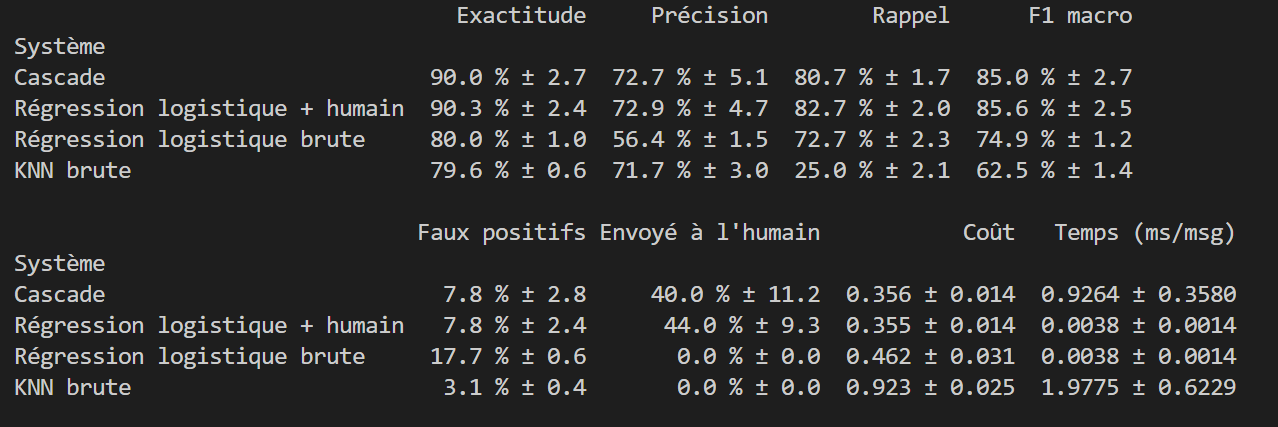
\includegraphics[width=\linewidth]{capture_terminal.png}
\caption{Sortie du terminal de \texttt{comparaison.py}.}
\end{figure}}{}

%% ===== CRÉDITS AUTEURS =====
\printcredits

%% ===== BIBLIOGRAPHIE =====
\bibliographystyle{cas-model2-names}
\bibliography{cas-refs}

\end{document}